\subsection{Thrust 2: Execution Stitching}
\label{sec:thrust2}

In this thrust, we will develop new techniques to reproduce concurrency bugs, which are complex bugs that can take weeks to fix~\cite{concurrencyAtMicrosoft}. \textbf{\textit{We will focus on bugs in highly-concurrent systems and long-running executions that were overlooked by the state of the art~\cite{h3,snorlax,rept}}}. We will augment trace-driven and adaptive symbolic execution to perform schedule exploration in a tractable way by using execution information from productions runs. We will achieve this by determining how key events (e.g., shared memory accesses) in reconstructed executions from Thrust 1 could interleave (be \textit{stitched} together) to yield to concurrency bugs. 

\noindent \textit{\textbf{Related Work}} A few techniques are geared towards \textit{detecting} concurrency bugs in production systems, such as deadlocks~\cite{jvmdeadlock,jstack} and data races~\cite{racemob}, however, to our knowledge, there is no effective technique currently deployed in production for \textit{reproducing} concurrency bugs. The difference is crucial: one can detect the presence of a deadlock, however, reproducing the execution and the schedule leading to the deadlock is more challenging. Unsurprisingly, reproducing the deadlocking execution is more useful, because then the developer can understand the conditions that led to it and craft an appropriate fix. REPT~\cite{rept} uses a coarse grain timer~\cite{snorlax} to infer the order of shared memory accesses that might cause a failure, however, if the timer granularity is insufficient, it discards the effects of shared memory operations, lowering its accuracy.

\noindent \textit{\textbf{Preliminary Work.}} We explored whether we could leverage H3~\cite{h3}, which uses constraint solving to determine the schedule of shared variables~\cite{clap} that causes a concurrency bug in the confines of a control flow trace. This is limiting, since capturing the \textit{entire} control flow (even with Intel PT~\cite{intelpt}) can incur up to 23\% overhead~\cite{h3}, which is not suitable for a production system. However, more importantly, as the authors point out, H3 may not scale to long-running executions with many read/write operations~\cite{h3}. To evaluate this, we randomly chose 10 latent concurrency bugs from our study~(\S\ref{sec:preliminary}). The buggy executions contain anywhere from 15-273 million instructions. We further determined the number of pairwise ordering constraints of shared memory read/write operations across threads to be between $\sim$8 million to $\sim$16 billion, which is up to six orders of magnitude greater than the largest number of constraints H3 was able to handle~\cite{h3}.

\subsubsection{Task 2.1: Hybrid Concurrency Bug Detection}
\label{sec:task21}
In this task, we will detect \textit{potential} concurrency bugs using a new hybrid static/dynamic analysis. Detection results may not be fully accurate, since to ensure \textit{efficiency}, we will use minimal information (e.g., core dump). We will improve accuracy in the next tasks.

\noindent \textit{Deadlocks.} Deadlocks can be identified by runtime~\cite{jvmdeadlock,windowswaitchain} support. We will use a similar post-mortem analysis to determine the locks involved in a deadlock to perform bug reproduction in T2.3 (\S\ref{sec:task23}).

\begin{wrapfigure}{L}{0.31\textwidth}
\centering
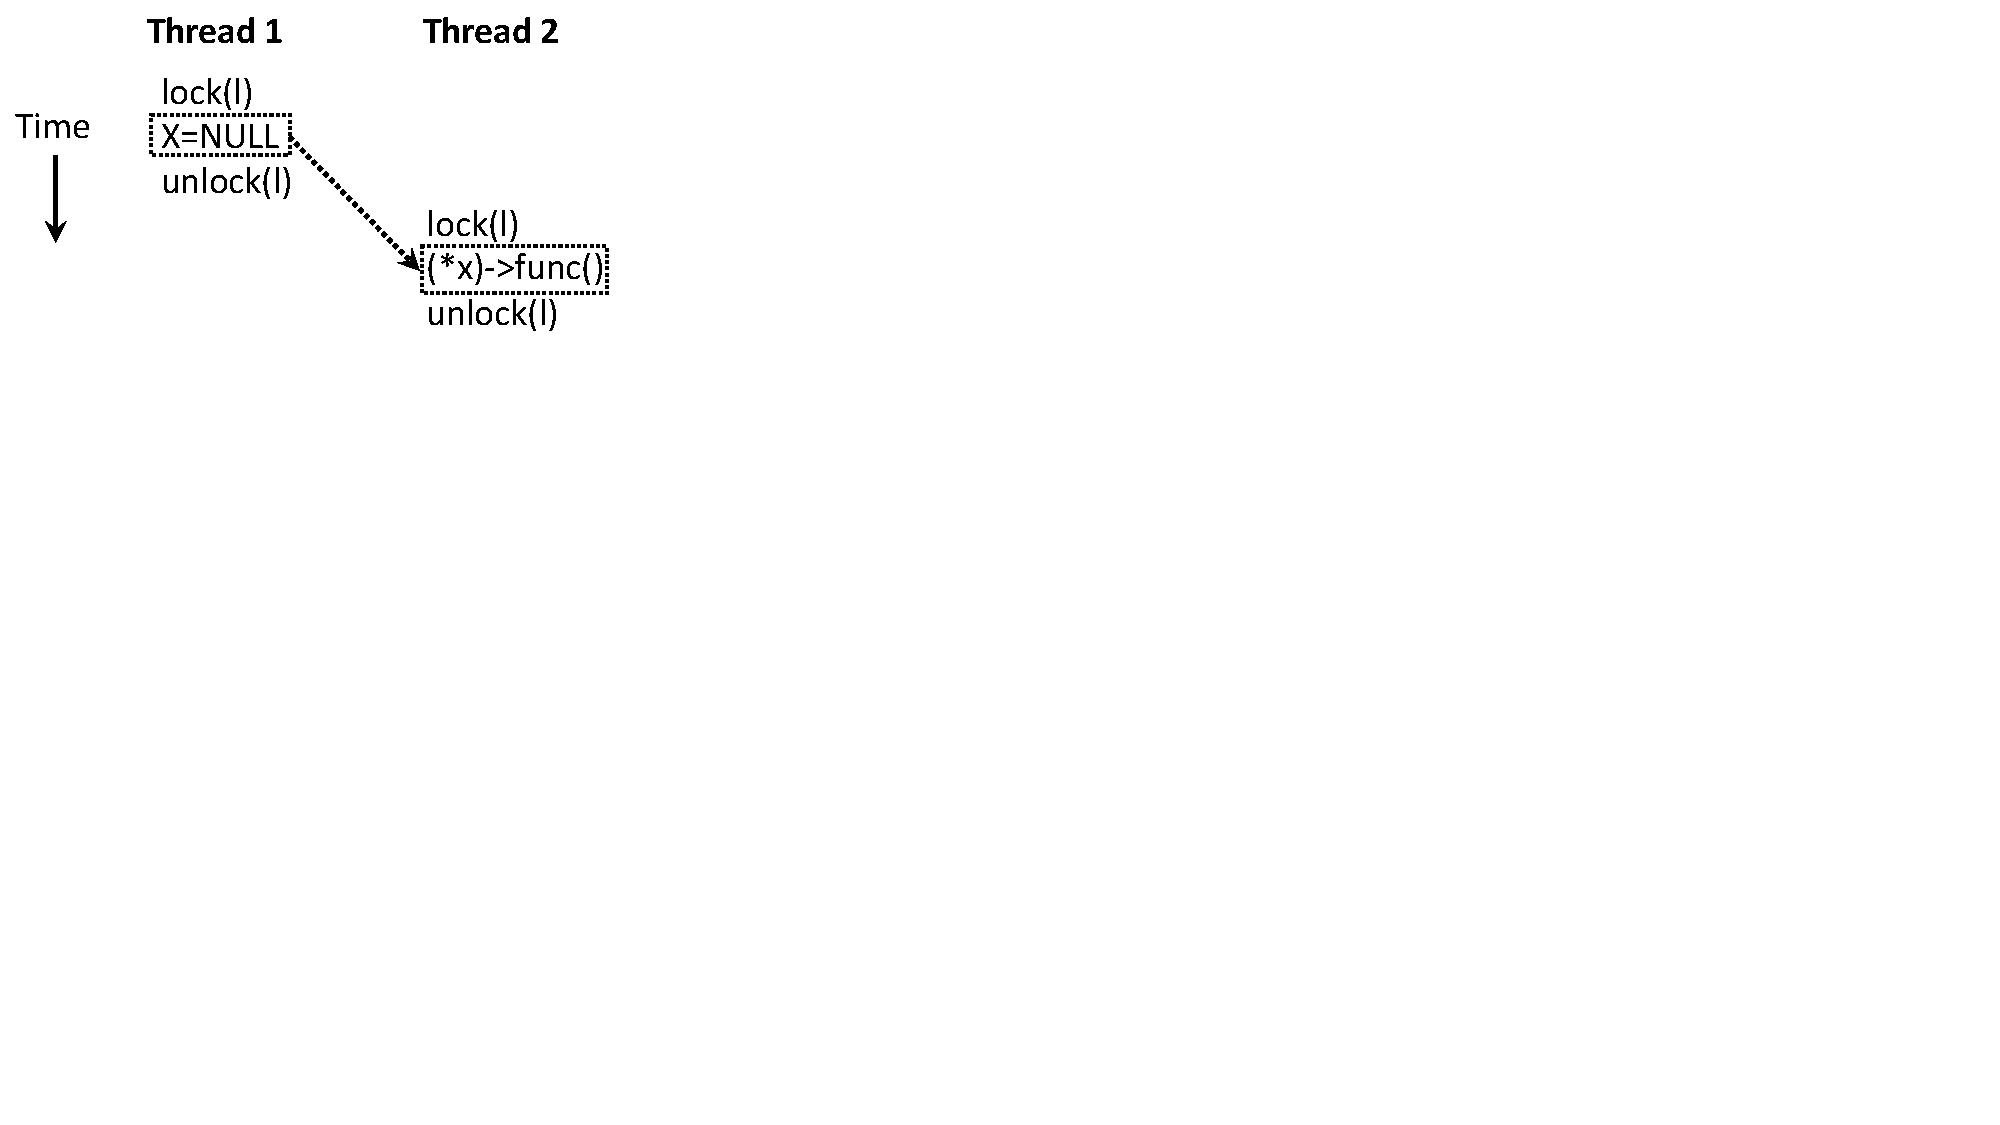
\includegraphics[width=\linewidth]{Figures/orderviolation.pdf}
\caption{Order violation, no race}
\label{fig:orderviolation}
\end{wrapfigure}

\noindent \textit{Data Races, Order Violations, and Atomicity Violations.} It is possible for order and atomicity violations to occur without an underlying data race~\cite{avio}. In Fig.~\ref{fig:orderviolation}, accesses to the shared variable x are protected by a lock (i.e., a happens-before relationship), so there is no data race, but the order of accesses causes a failure. However, we make a \textit{\textbf{design decision}} to prioritize reproducing concurrency bugs with an underlying data race, because factoring happens-before relationships in concurrency bug detection to reduce the number of schedules to explore greatly reduces complexity, and we posit that \textit{majority} of concurrency bugs have an underlying data race (see preliminary work below). 

 We will statically detect \textit{potential} data races in house (offline). The verdict is potential, because the algorithm may think that the racing instructions: (1) \textit{may} (not \textit{must}) be accessing the same memory location as determined via alias analysis, (2) are from different threads, (3) are not ordered by a happens-before relationship (e.g., lock/unlock, signal/wait, etc.). To detect data races, we will modify an existing algorithm~\cite{relay} to use our interprocedural pointer analysis from T1.1 (\S\ref{sec:task11}). The analysis will also determine synchronization operations (known ones like the pthread API, as well as custom ones that developers may specify) that operate on the same synchronization variable (e.g., a lock instance). For non-LLVM environments, we will use either another existing static data race detector~\cite{locksmith} or rely on binary-to-llvm conversion~\cite{revnic,mctoll}.

When a program fails in production, we will attempt reconstructing an execution with no regard to the thread schedule (e.g., as in Thrust 1). Many bugs are sequential, and even concurrency bugs can be reproduced fortuitously. In this thrust, we will augment the control flow trace gathered in production to also include timing packets (supported by Intel PT~\cite{intelpt} and ARM ETM~\cite{armetm}). These packets provide a coarse-grained timer ($\sim$20 usec) that allows ordering events in traces gathered from different threads.

%~\footnote{E.g., in Intel PT, the original trace is per-core, however with proper driver support~\cite{snorlax} we can gather per-thread traces.} 

We will simultaneously initiate hybrid concurrency bug detection. First, we will use the data values in the core dump to soundly discard accesses that were not made to the same memory location. These accesses may be made to the same memory location in \textit{some} execution, but we know that in the \textit{failing execution}, they were not. Similarly, we remove from the results synchronization operations that were not accessing the same variable (e.g., the lock instance). Since the control flow traces are per-thread, we will also discard pairs of accesses made from the same thread. Finally, if static analysis can conclusively identify the synchronization variable, (which is likely, since synchronization variables have distinct types, so alias analysis works well), we will use the timing information in the control flow traces to infer happens-before relationships in the failing execution. We will use these relationships to help adaptive schedule synthesis in T2.3~(\S\ref{sec:task23}). We will also determine accurate aliasing information by tracking the addresses accessed in successful executions using hardware support (PT\_WRITE) like we proposed in T1.2~(\S\ref{sec:task12}).

\noindent \textit{\textbf{Preliminary work.}} To assess the implications of our decision to focus on concurrency bugs caused by data races, we analyzed all the 86 order and atomicity violations and found that only 3 of them (3.4\%) are not caused by a data race, suggesting that even if we cannot reproduce such bugs, our effectiveness will be high. 


%Intel CPUs since Nehalem have invariant TSC~\cite{intel:sdm}, meaning that the TSC is synchronized across the CPUs~\cite{tsc-sync}

\subsubsection{Task 2.2: Schedule Refinement via Adaptive Monitoring} 
\label{sec:task22}

Hybrid data race detection (T2.1, \S\ref{sec:task21}) can have inaccuracies due to static analysis, causing a large number of interleavings to explore to reproduce concurrency bugs. We will use the interleavings of key events (shared memory accesses and synchronization operations) in successful production executions to build a \textit{successful interleaving profile}. Our novel idea is to steer the exploration of concurrency bugs towards interleavings that are outside this profile (T2.3, \S\ref{sec:task23}). The key insight, as observed by us and others~\cite{kasikcithesis,arulraj:pbi,jin:cci,snorlax,gist} is that the interleaving of key events like memory accesses is the defining trait of concurrency bugs. In other words, a buggy interleaving tends to always lead to a failure and a successful interleaving does not (see preliminary work below).

\begin{wrapfigure}{R}{0.23\textwidth}
\centering
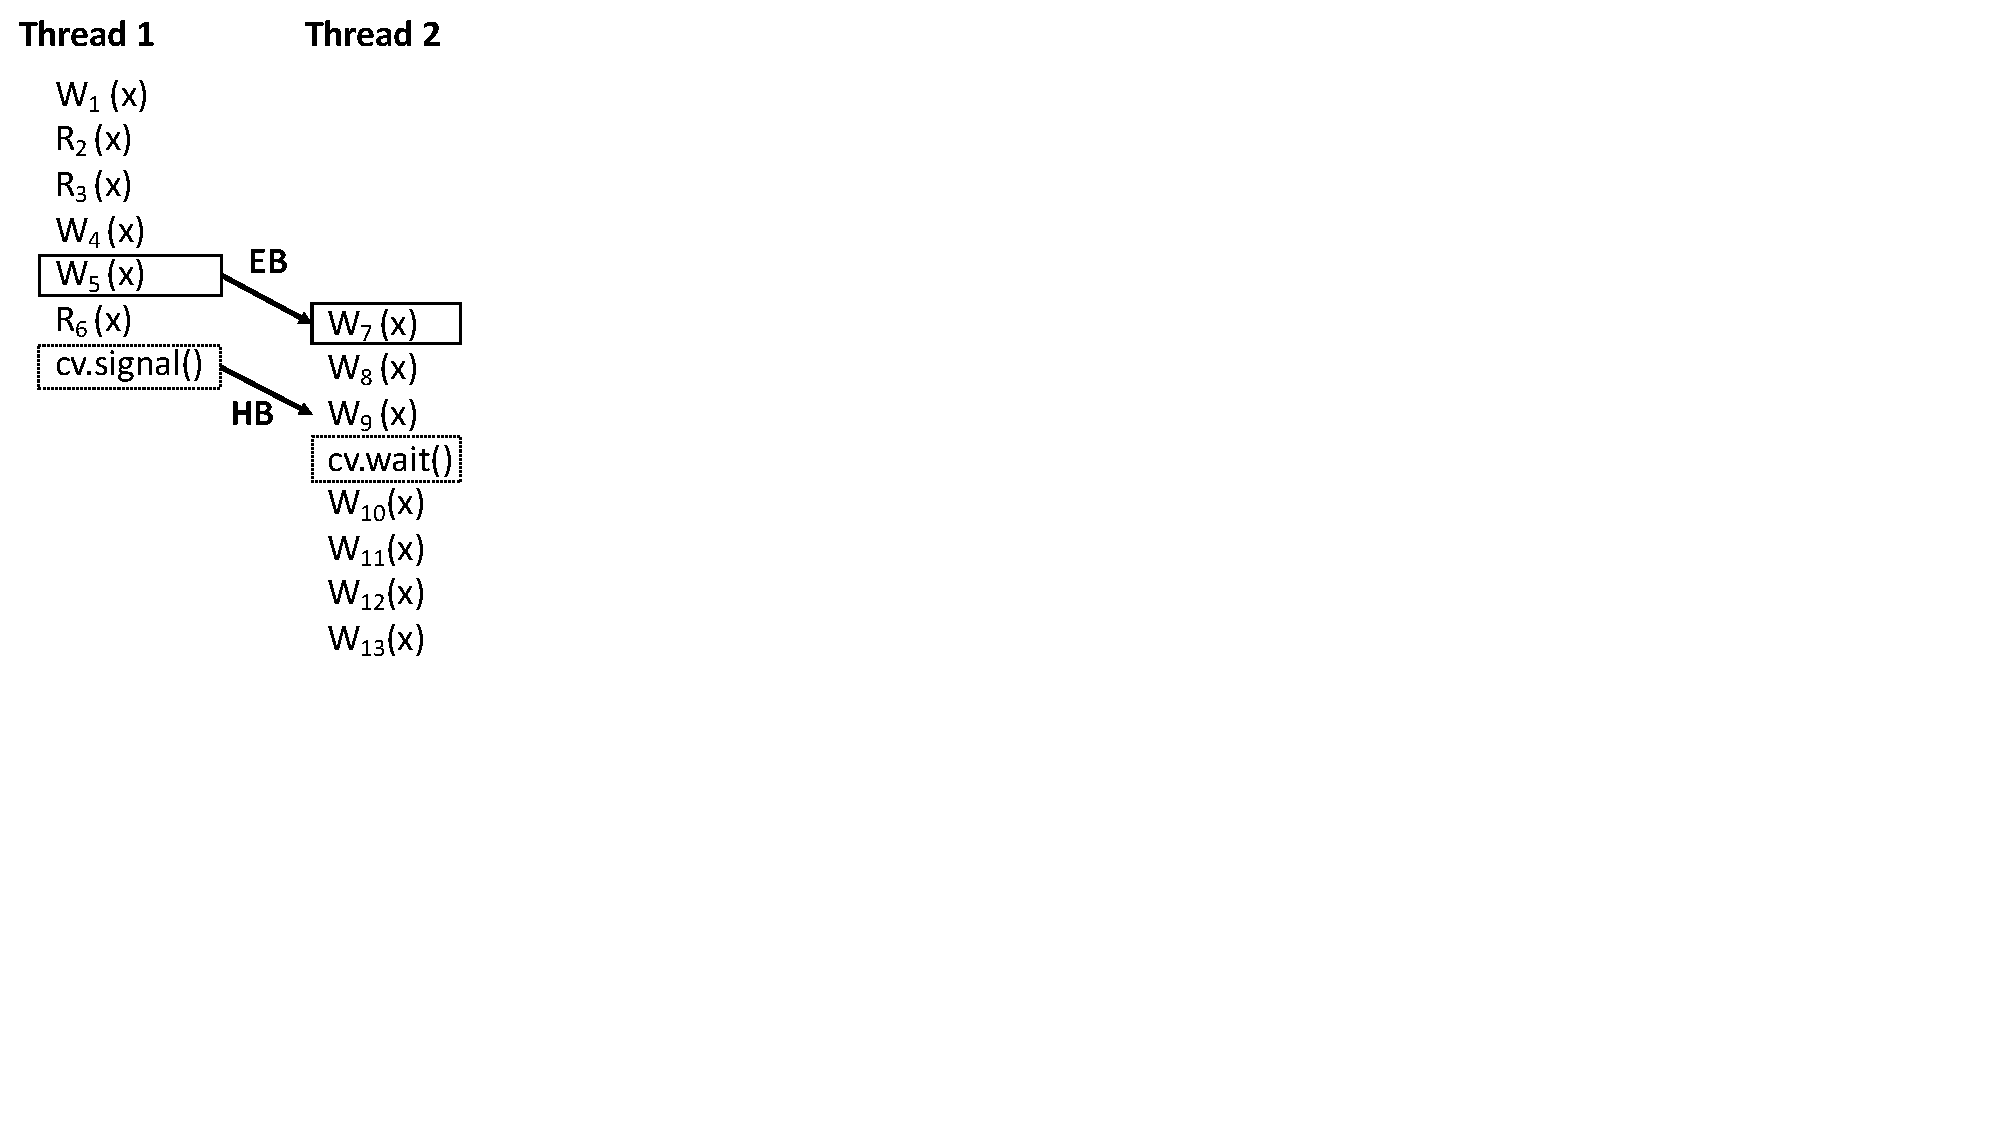
\includegraphics[width=\linewidth]{Figures/reduction.pdf}
\caption{Exclusion of successful interleavings}
\label{fig:reduction}
\end{wrapfigure}

To see how identifying the interleavings of synchronization operations and shared memory accesses of successful executions can help with bug reproduction, consider Fig.~\ref{fig:reduction}, where W(x) and R(x) denote a write to and a read from a shared memory location x and the events \textit{within} a thread are totally-ordered. HB represents a happens-before relationship~\cite{lamporthb} and EB represents a relation we call \textit{executes-before}~\cite{snorlax}, which is based on the timestamps in the control flow trace. Further, assume that this is a successful execution. If we discard HB and EB relationships, there are potentially 6 ($W_1...R_6$) x 7 ($W_7...W_{14}$) = 42 pairs of racing accesses, whereas if we factor them in, the number of racing pairs reduces to 2 ($R_6-W_8$ and $R_6-W_9$). The EB relationship does not imply an HB relationship, however, since this is a successful execution, we will use it to build the successful interleaving profile and steer concurrency bug detection towards different interleavings. If bug reproduction is unsuccessful, we can discard the EB relationship and explore resulting interleavings with potential data races.

We will infer executes-before relationships using timestamps in the control flow traces as in our prior work, which is effective in many cases~\cite{snorlax}. However, inferring happens-before relationships is more challenging to achieve with these coarse-grained timestamps (see preliminary work below), yet crucial, since they substantially reduce the interleaving space to explore.

\begin{wrapfigure}{L}{0.27\textwidth}
\centering
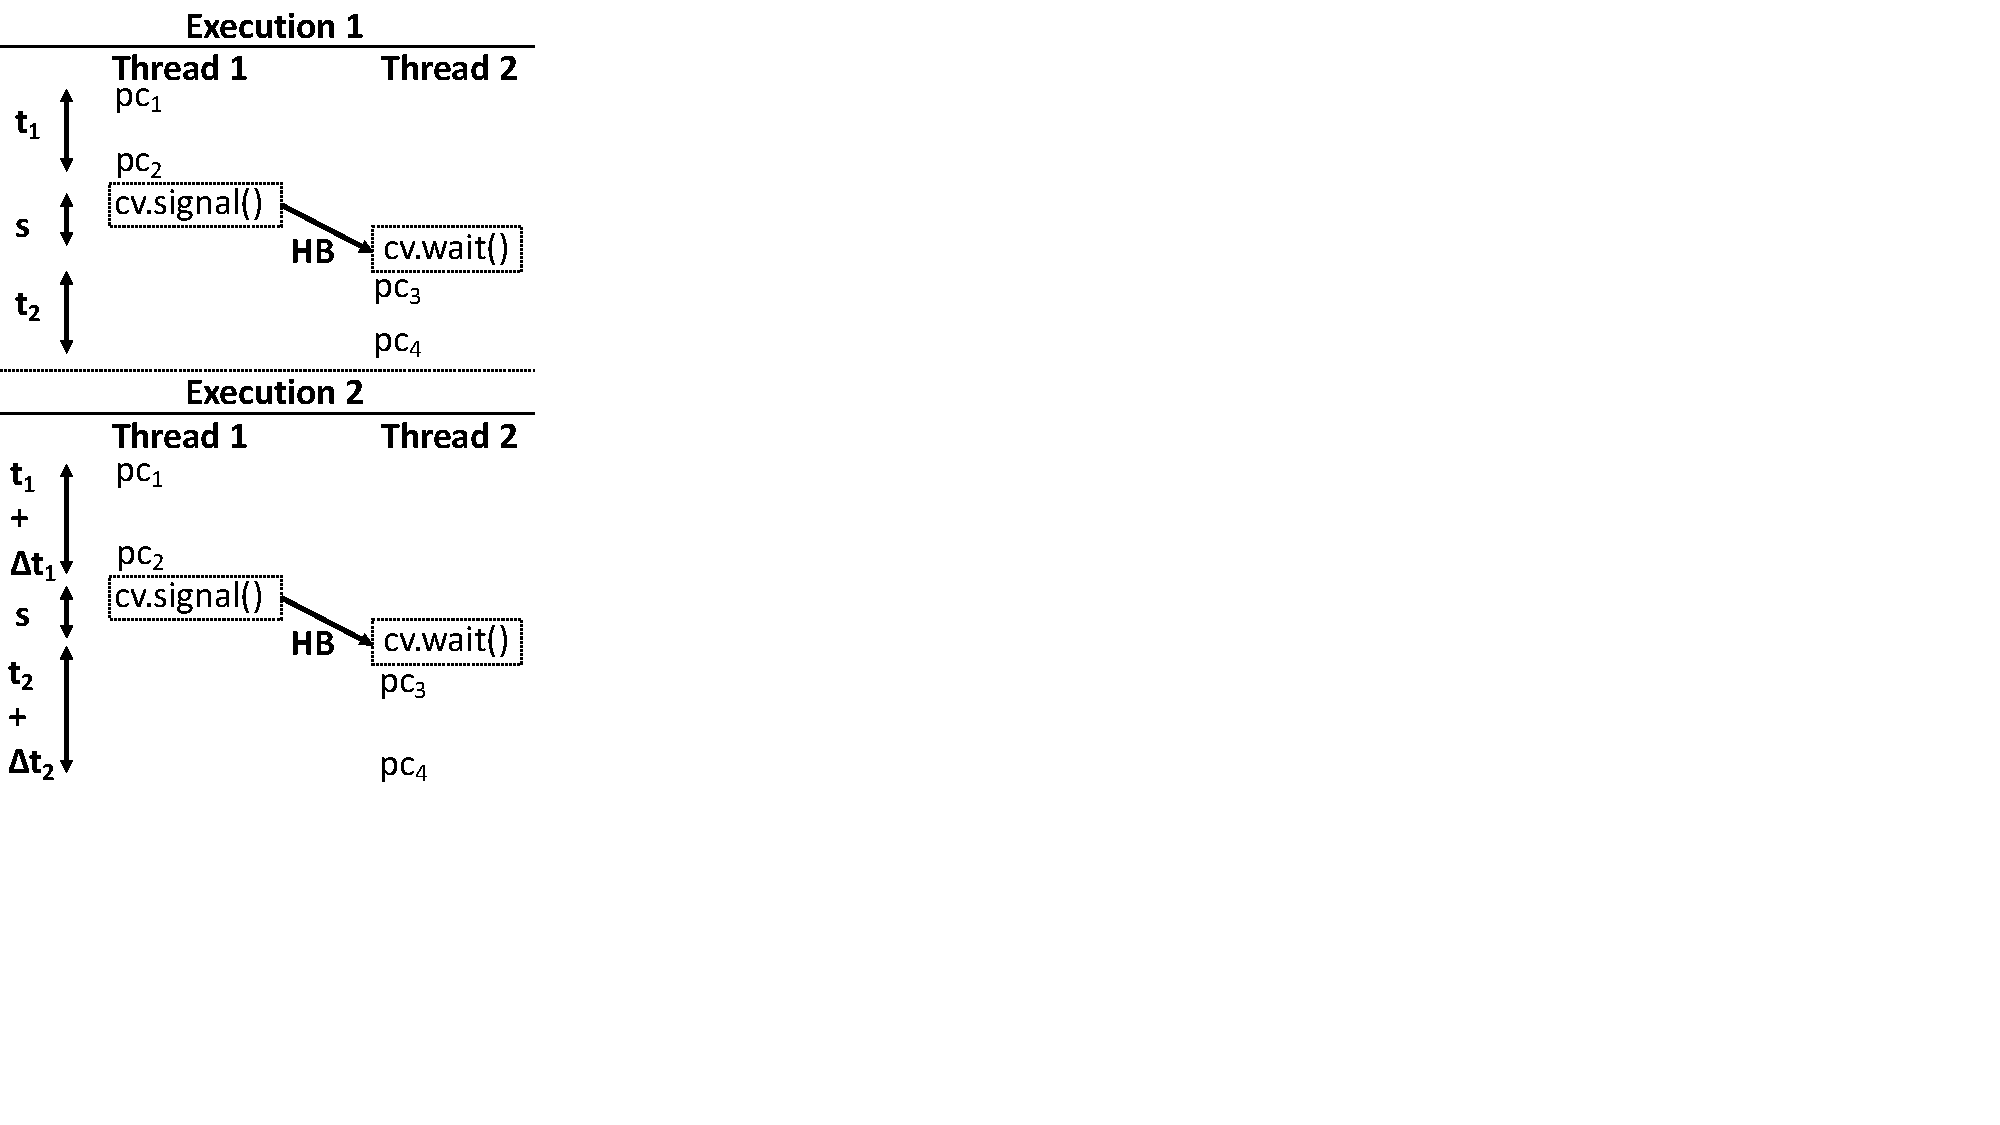
\includegraphics[width=\linewidth]{Figures/amplification.pdf}
\caption{Clock amplification}
\label{fig:amplification}
\end{wrapfigure}

To solve this challenge, we will introduce a novel technique called \textit{\textbf{clock amplification}}. The key idea is to observe the effects of happens-before relationships on portions of an execution that can be timed with a coarse-grained timer. Consider Execution 1 in Fig.~\ref{fig:amplification}, where the time elapsed between the execution of program counters $pc_1,pc_2$ and $pc_3,pc_4$ is $t_1$ and $t_2$ respectively. The time elapsed between the signal and the wait is $s$. We assume that the granularity of timestamps is too coarse to measure $s$, but it is sufficient to measure $t_1$ and $t_2$, which is easily achieved since we get to pick $pc_1...pc_4$. We will use region monitoring facilities in Intel PT and ARM ETM to collect control flow traces with timestamp information between $pc_2-pc_1$ and $pc_4-pc_3$. In Execution 2, the time elapsed during these program portions is $t_1 + \Delta_{t_1}$ and $t_2 + \Delta_{t_2}$. We argue that this variation in time will naturally occur in a program (e.g., due to cache behavior, I/O throughput, network latency, etc.). Our observation is that if $\Delta_{t_1}$ and $\Delta_{t_2}$ have a similar value (in a statistically-significant way), then, there is potentially a happens-before relationship between the portions $pc_1-pc_2$ and $pc_3-pc_4$. We will use this heuristic to guide schedule exploration. 

To improve efficiency, we will \textit{adaptively} alter the regions we monitor using clock amplification. \textit{\textbf{The adaptive strategy will prioritize inferring happens before relationships that can quickly reduce the schedule space to explore}}, which is critical especially when programs employ heavy multithreading. 

\noindent \textit{\textbf{Preliminary Work.}} We analyzed the 246 concurrency bugs from our study. All of them were caused due to a specific interleaving and can be avoided by modifying the interleavings, which motivates our heuristic that prioritizes interleavings that do not occur in successful executions. We also measured the time elapsed during synchronization operations (e.g., signal-wait) and determined that they take 1 to 3 microseconds, suggesting that a coarse-grained timer like Intel PT's ($\sim$20 usec) cannot be used to determine such happens-before relationships. Finally, to test whether clock amplification is a viable technique to infer happens before relationships, we used SQLite and instrumented two program portions, one before and one after a lock operation ({\tt \small pagerLockDb/pagerUnlockDb}) to measure time elapsed when running the SqLite tests~\cite{sqlitetests}, which exercised the monitored code 100 times. 92/100 times, the time difference in the first portion ($\Delta_{t_1}$ above) was within 95\% of the time difference in the second portion ($\Delta_{t_2}$ above) and the time difference was at least 110 usec, suggesting a coarse grain timer can be used.
 
% racerx,locksmith 

%The common theme across all these bug sub-classes is access to shared data. As a result, we will rely on an interprocedural static analysis to determine shared data. Since there is no precise notion of threads during static analysis, this analysis will rely on alias analysis to determine memory locations that are potentially accessed by multiple program locations. Atomicity violations, deadlocks, and in some cases order violations, further involve accesses to synchronization primitives such as locks and condition variables. Our static analysis will also detect synchronization variables (and how they are shared and used) based on the existing knowledge of synchronization primitives (e.g., {\tt \small pthread\_lock} in C/C++, {\tt \small synchronized} in Java). 

%If developers use custom (ad-hoc) synchronization, they will be able to provide this as an input for the analysis, but we don't rely on this to reproduce bugs.


\subsubsection{Task 2.3: Symbolic Schedule Synthesis} 
\label{sec:task23}


\begin{wrapfigure}{R}{0.37\textwidth}
\centering
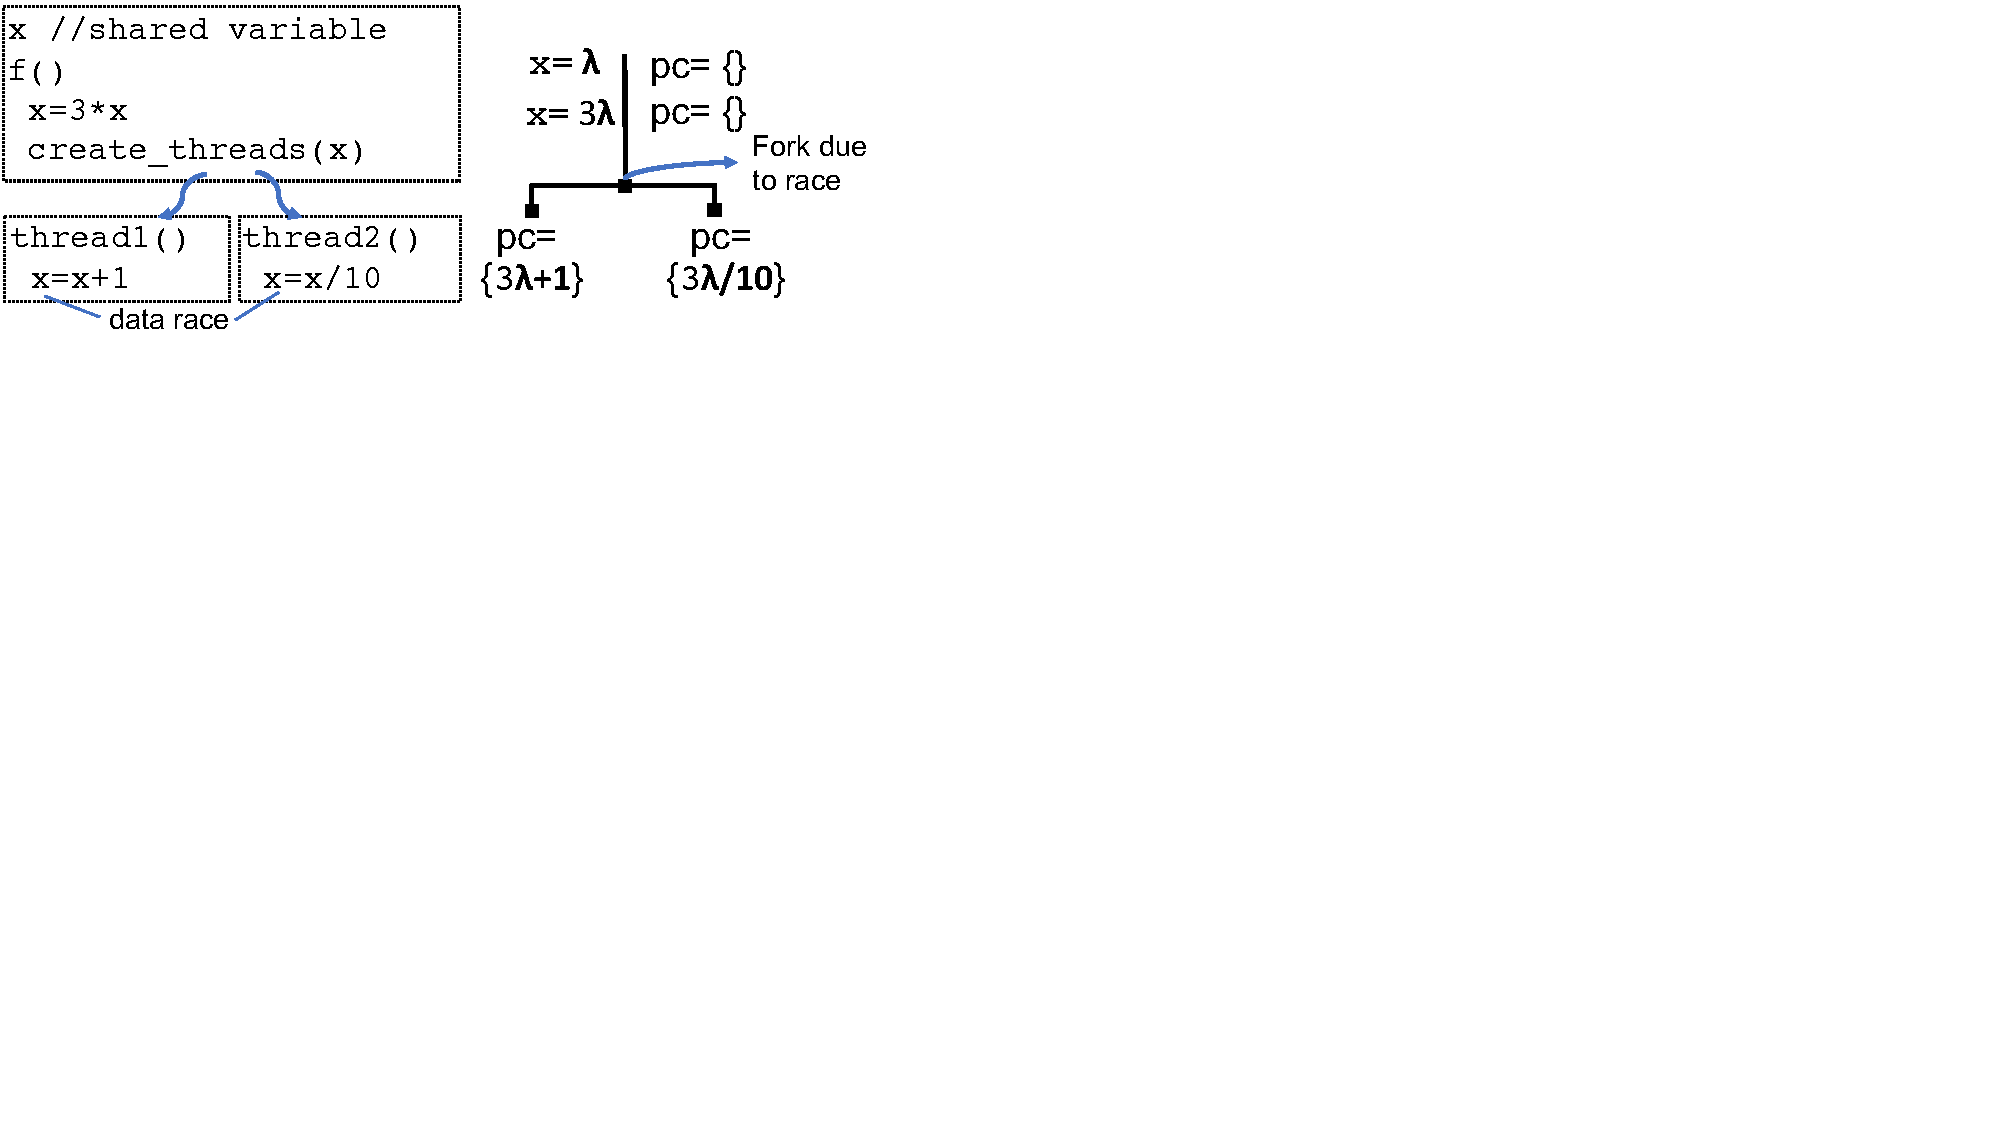
\includegraphics[width=\linewidth]{Figures/s3.pdf}
\caption{Schedule synthesis}
\label{fig:s3}
\end{wrapfigure}

In this task, we will develop a new technique called \textit{Symbolic Schedule Synthesis} ($S^3$) that augments adaptive symbolic execution (T1.3, \S\ref{sec:task13}) to account for thread schedules. $S^3$ forks symbolic execution along the hybrid slice whenever a potentially racing shared variable is encountered. As opposed to work that treats schedules as separate constraints~\cite{h3,portend}, this approach will express scheduling decisions in terms of their effect on shared variables. In Fig.~\ref{fig:s3}, {\tt \small x} is a shared variable accessed by threads 1 and 2. Since both threads update x with no intervening synchronization, there is a data race. The symbolic execution tree shows how this data race triggers a fork (see~\S\ref{sec:background}). To reproduce deadlocks, $S^3$ forks the execution at lock operations determined to be involved in a deadlock (T2.1, \S\ref{sec:task21}). In this case, $S^3$ forks the program state and executes a particular lock operation. There is no need to maintain a scheduling constraint as the acquisition of the lock models the execution behavior that $S^3$ is trying to explore (i.e., how a deadlock is reached through the successive acquisitions of locks). Expressing scheduling constraints in terms of their effects on variables eliminates redundancy in path constraints and creates \textit{more compact} constraints. There is no further need to maintain scheduling constraints in their own \textit{domain}, and the resulting path conditions will contain fewer disjunctions, which are difficult for SAT solvers~\cite{statemerging}.

\noindent \textit{\textbf{Prior and Related Work.}} We previously built a multithreaded symbolic execution engine that keeps track of scheduling decisions separately (e.g., $pc_1 \wedge (Thread_1 \vee Thread_2)$). Others built symbolic execution engines for data-race-free programs~\cite{symbexmt}, which do not help reproduce concurrency bugs. 

%Concolic execution of multithreaded programs~\cite{senconcolicmt} relies on a concrete inputs (which we do not assume to have access) reproduce data races and generate test cases by flipping the execution orders of racing accesses.

\noindent \textit{\textbf{Preliminary Work.}} To evaluate if $S^3$ can reduce constraint complexity, we symbolically executed pbzip2~\cite{pbzip2}, a compression tool, for one hour using ESD~\cite{esd} with symbolic inputs. We chose pbzip2, because we have studied it in the past and know the data races it contains. We then analyzed the generated constraints to see that 41\% of the constraints across all clauses pertain to scheduling decisions, which will be eliminated with our approach. To approximate the effect of this on solving time, we assumed that every scheduling constraint holds true. We compared the constraint solving time of this configuration to the baseline solver time (i.e., with the thread scheduling constraints) at a random program location after one hour and saw a 23$\times$ reduction, which is encouraging.

\subsubsection{Potential Challenges and Mitigation Strategies}
\label{sec:mitigation2}

Certain concurrency bugs occur without an underlying data race. If these bugs become more prevalent, we can tailor our static analyses to recognize their underlying patterns. We might also explore using hardware support such as recent cache-coherent shared memory FPGA/CPU platforms (e.g., Intel HARP). We can implement a monitoring algorithm to efficiently detect these code patterns executing on the CPU by leveraging the FPGA. We will explore this direction with Intel's support and access to upcoming hardware through Intel vLab~\cite{vlab} (see attached letter from Intel).

% full participation of women, persons with disabilities, and underrepresented minorities in science, technology, engineering, and mathematics (STEM); improved STEM education and educator development at any level; increased public scientific literacy and public engagement with science and technology; improved well-being of individuals in society; development of a diverse, globally competitive STEM workforce; increased partnerships between academia, industry, and others; improved national security; increased economic competitiveness of the United States; and enhanced infrastructure for research and education.